Last day! I'm flying out this afternoon so I will only make a few sessions today.


\subsection{Contributed Talks}

Now some contributed talks.

\subsubsection{Felix Wiu on Pay Less Attention with Sequence Models~\cite{wu2019pay}}

{\bf Observation:} Sequence models are almost everywhere in NLP (have become the CNN$\leftrightarrow$ vision). \\

This work:
\begin{enumerate}
    \item Q1: Is self attention needed for good performance?
    \item Q2: Can we do well on a range of NLP tasks with limited context?
\end{enumerate}

Different models perform very differently on Neural machine Translation (Transformer achieve BLEU of 28, SliceNet of 25, phrase-based of 22). \\

$\ra$ Large performance gap of self-attention and convolutional models. \\

Background: three ways to encode a sequence
\begin{itemize}
    \item RNN: recurrent neural net.
     can.
    $h_t = f(x-t, h_{t-1})$, with $x_i$ the input at time $i$, $h_i$ the hidden state at time $i$.
    
    \item CNN: convolutional neural net.
    
    $h_t = f(x_{t-k}, \ldots, x_{t+k})$ $\ra$ look at a limited window.
    
    \item Self-attention models: Compute pairwise similarity between words and aggregate them.
    
    $h_t = \sum_{i,j} a_{i,j}$.
\end{itemize}

Some pros and cons of each! RNNs can't be parallelized, while CNNs and self-attention, time complexity is higher for self-attention, and so on (see Figure~\ref{cnn_rnn} for full comparisons). \\

\begin{figure}[h!]
    \centering
    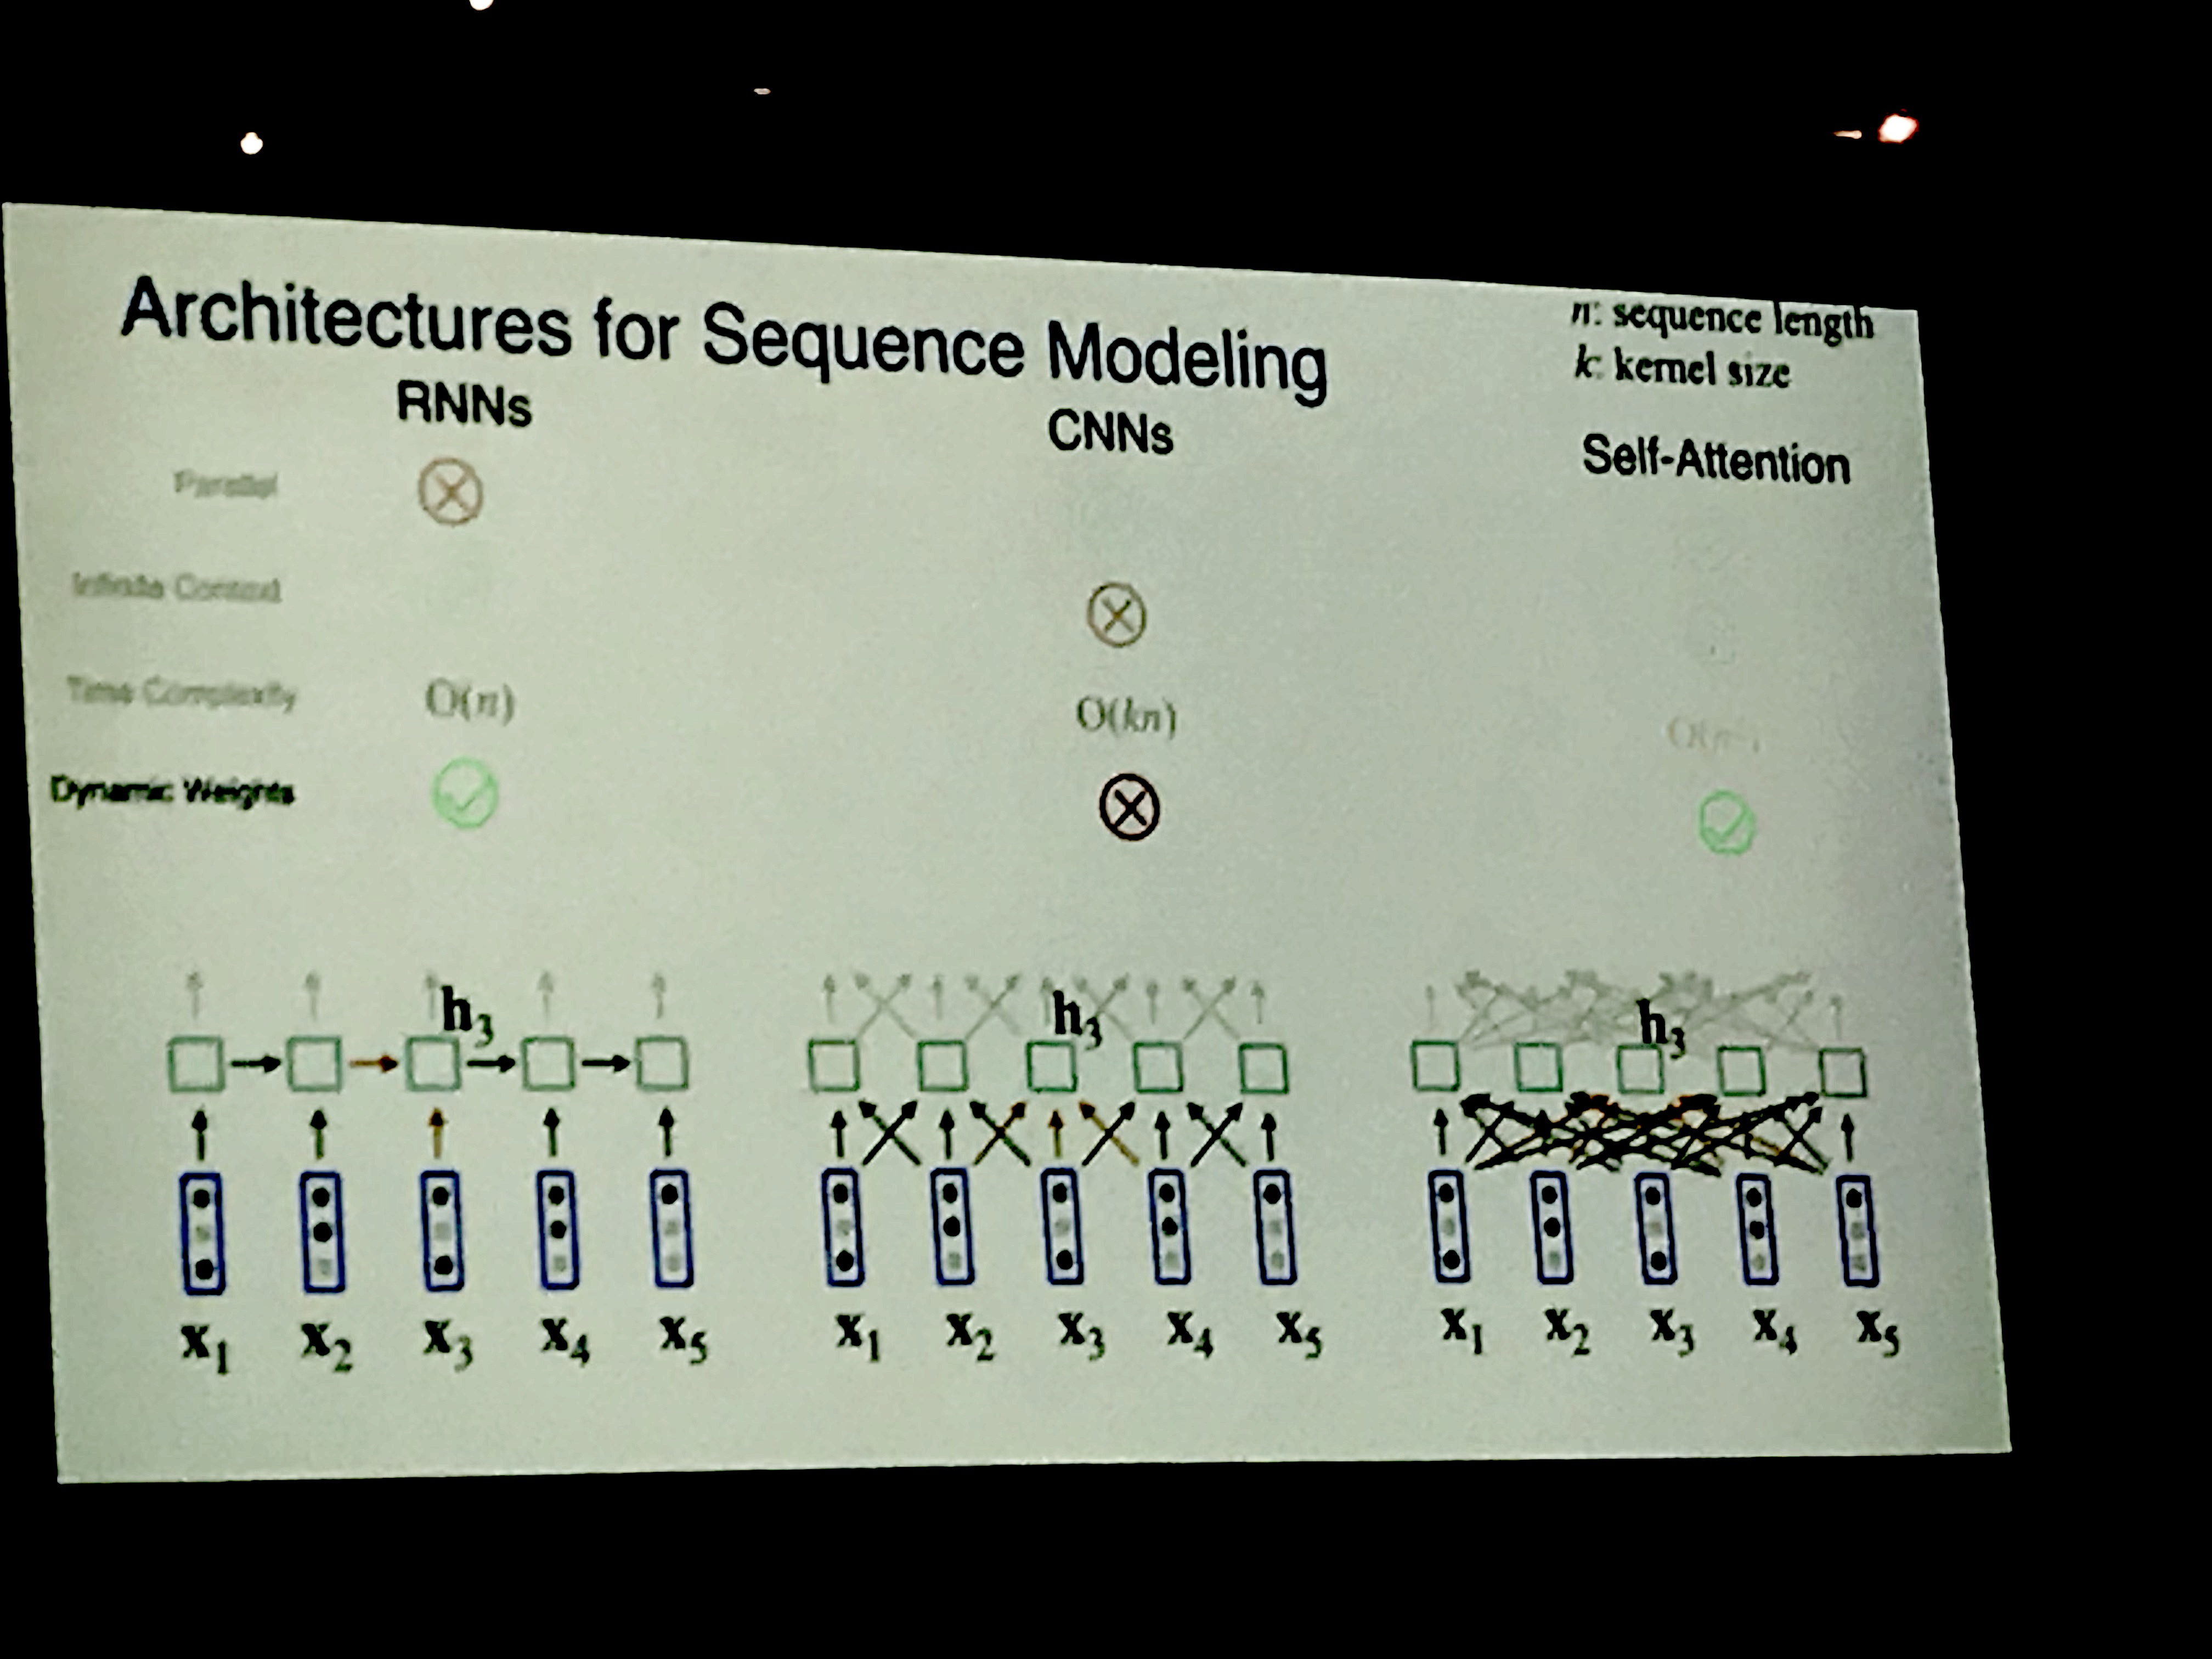
\includegraphics[width=0.4\textwidth]{images/cnn_rnn-2.JPG}
    \caption{Pros and Cons of CNNs, RNNs, and self-attention for sequence modeling.}
    \label{fig:cnn_rnn}
\end{figure}

{\bf Approach:} {\it dynamic} convolution that addresses the main disadvantage of CNNs (lack of dynamic weighting). \\

But, some challenges to dynamic convolution: too many parameters to optimize! \\

$\ra$ Response: turn to lightweight convolution, which reduces the number of parameters. \\

{\bf Experiments:} Explore the trade-off made between {\it inference speed} measured by sentences per second) vs. {\it BLEU score}, which is a way to measure the quality of output translations. \\

$\ra$ Main finding: dynamic convolution achieves same BLEU score as self-attention, but with a 20\% speed up in inference time. \\

Conclusion:
\begin{enumerate}
    \item Local information is sufficient for several NLP tasks.
    \item Introduced dynamic convolution: context-specific kernels.
    \item Lightweight convolution: fewer convolution weights still work well.
\end{enumerate}


\subsubsection{Jiyauan Mao on Neural-Symbolic Context Learner~\cite{mao2019neuro}}

{\bf Focus:} Visual concept reasoning. \\

$\ra$ Given an input image (of some objects), people can quickly recognize the objects, texture, surface, and so on. \\

Visual Question Answering: given an image and a question ``What's the shape of the red object?", output an answer to the question. \\

$\ra$ Also, may want to do image captioning: ``there is a green cube behind a red sphere", or instance retrieval (a bounding box on a particular object). \\

{\bf Prior Approaches:} End-to-end approaches for solving these three problems. Two things to learn: 1) concepts (colors, shapes), and 2) reasoning (counts). \\

$\ra$ Downside to end-to-end: concept learning and reasoning are entangled. Not obvious how to transfer. \\

{\bf This Approach:} Incorporate concepts in visual reasoning. Prior methods rely on excpliti concept annotation. \\

The idea:
\begin{itemize}
    \item Joint learning of concepts and {\it semantic parsing}.
    \item Given a scene parser, and a semantic parser, learn a program that understands the concepts while parsing both objects.
\end{itemize}

Example: given an image of a red sphere and green cube, first perform object detection/feature extraction to get a representation. At the same time, do semantic parsing on the text, to output a parse program that predicts the output of the question. The full overview is given in Figure~\ref{fig:cube}

\begin{figure}[h!]
    \centering
    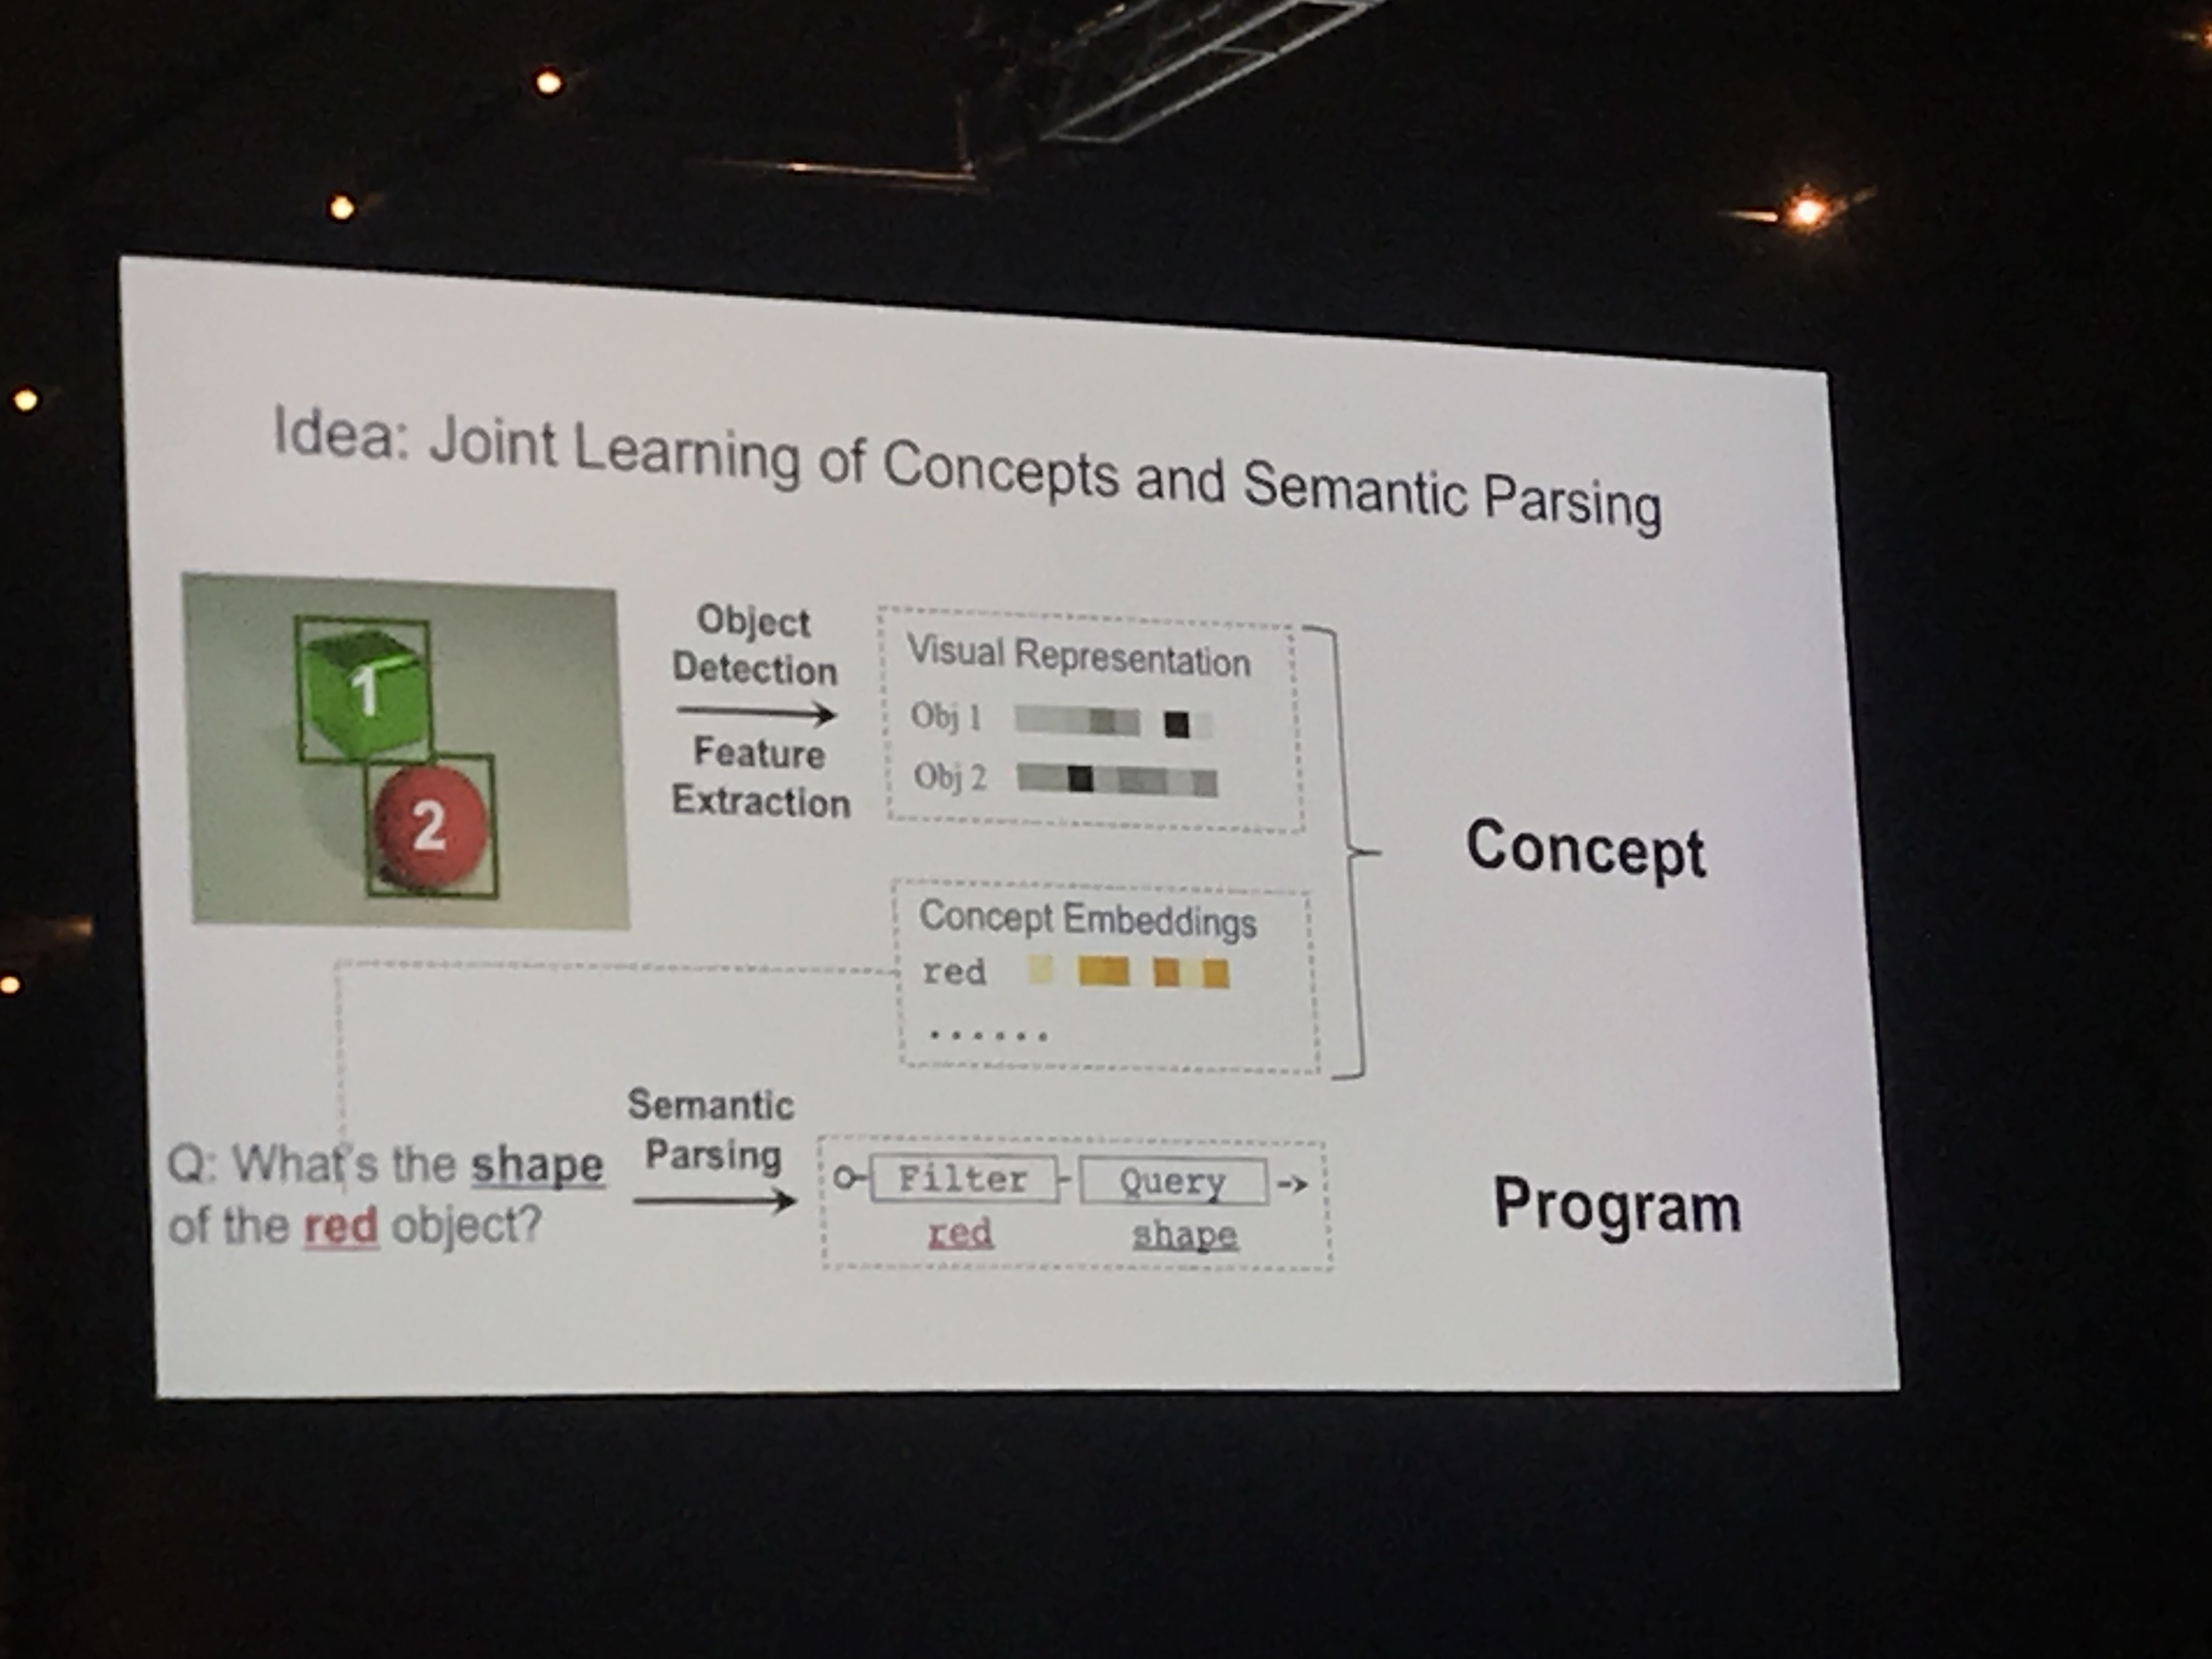
\includegraphics[width=0.4\textwidth]{images/cube.JPG}
    \caption{Overview of the approach for joint semantic and scene parsing.}
    \label{fig:cube}
\end{figure}

Two main methods:
\begin{itemize}
    \item Learn a program for understanding concepts
    \item Learn a concepts that can help facilitate parsing new sentences
\end{itemize}

{\bf Experiments:} This approach yields several advantages
\begin{itemize}
    \item State of the art performance on the "CLEVR" data set for visual question answering.
    \item Extensions to natural images and natural sentences as in the VQS dataset: ``what color is the fire hydrant?" given a natural seeming image of a fire hydrant (correctly guesses ``yellow").
    \item Model also supports composition of low level concepts into high level concepts, and bounding box detection.
\end{itemize}

{\bf Limitations and Future Directions:}
\begin{itemize}
    \item Consider example of a person with an umbrella hat on, and the question ``what purpose does the thing on this person's head serve"? proves extremely challenging!
    \item Recognition of in-the-wild images and beyond (like goals).
    \item Interpretation of noisy natural language
    \item Concept learning in a more sample efficient way.
\end{itemize}

Conclusions:
\begin{itemize}
    \item New model: NSCL learns visual concepts from language with no annotation
    \item Advantages of new model:  high accuracy and data efficiency, transfer concepts to other tasks.
    \item Principles: explicit visual grounding of concepts with neuro-symbolic reasoning.
\end{itemize}

\subsubsection{Xiang Li on Smoothing Geometry of Box Embeddings~\cite{li2018smoothing}}

{\bf Point:} Learning representations is crucial in NLP! These representations are usually vectors like word2vec or BERT. \\

$\ra$ These vectors define semantic similarity in space (closer together words have similar meaning/use). \\

But, consider: Rabbit/mammal. They're close to each other in space, but don't capture the full complexity of their relationship rabbit $\subset$ mammal). \\

$\ra$ One idea: Gaussian representation of classes like ``mammal". Advantages: 1) region, 2) asymmetry, 3) disjointness; but, one downside: not closed under intersection. Recent work extends this to a probabilistic model that gives up disjointness to achieve closure under intersection. \\

{\bf Their Approach:} An extension of these probabilistic models using a {\it box representation} to account for joint concepts, thereby achieving all four of the desired properties (region, asymmetry, etc.). Box representation seen in Figure~\ref{fig:box}. \\

\begin{figure}[h!]
    \centering
    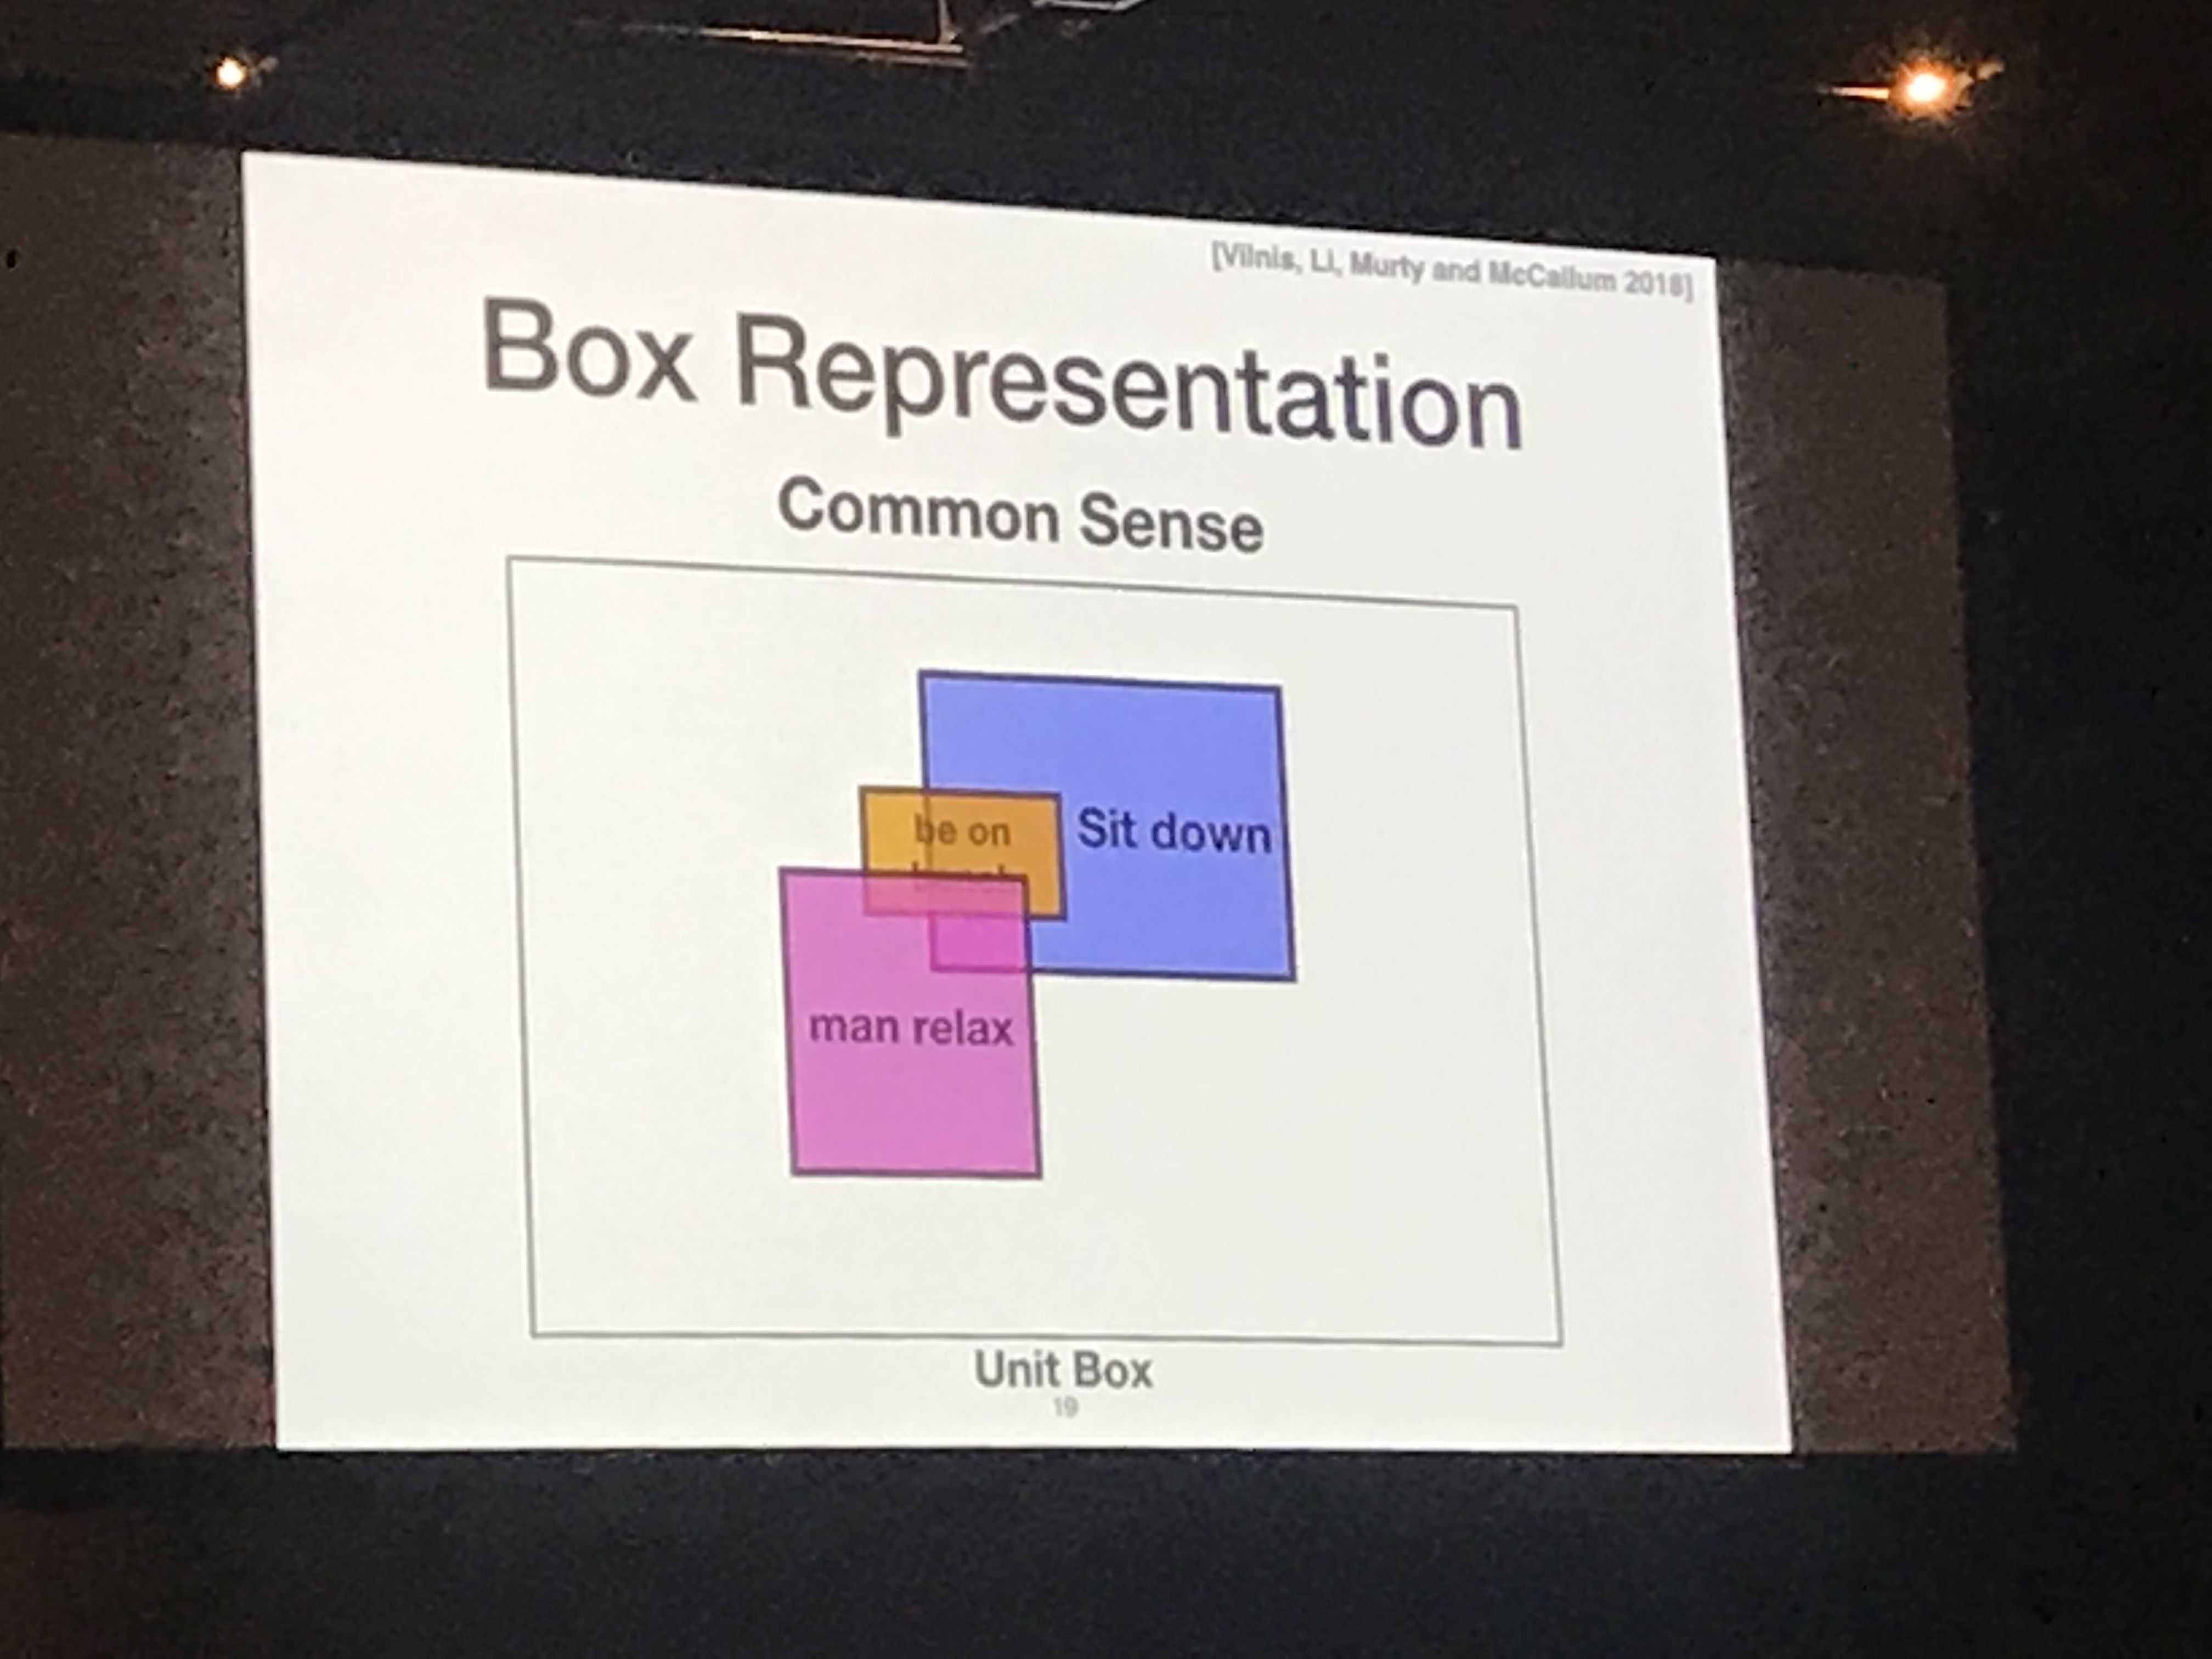
\includegraphics[width=0.4\textwidth]{images/box.JPG}
    \caption{Idea behind the new probabilistic box representation}
    \label{fig:box}
\end{figure}

Learning problem; boxes represent probability mass, try to do distribution matching over concepts. Initialize random concepts ($Pr(deer), Pr(deer \mid mammal)$. \\

{\bf Experiments:} 1) Matrix factorization in MovieLens, 2) Classification on Imbalanced Wordnet

\begin{enumerate}
    \item MovieLens Marketbase; Movie $\times$ Movie matrix: $p(lion king \mid aladdin) = 0.73)$, 286 million pairs.
    
    $\ra$ Regression task: train/dev/test, yields a matrix factorization problem (determine which movies people will like). \\
    
    $\ra$ Forrest Gump ends up being a large box, indicating that everyone likes it!
    
    \item Imbalanced WordNet: show the models learning ability for sparse, disjoint data.
    
    $\ra$ Binary classification task: achieve SOTA, even with sparse/disjoint data.
\end{enumerate}

\subsubsection{Best Paper Award Talk: Yiqang Shen on Ordered Neurons~\cite{shen2019ordered}}

{\bf Assumption:} Language has a latent tre-like structure \\

$\ra$ This work: focus on {\it constituency tree}. \\

Q: Why? \\

A1: Hierarchical representations with increasing levels of abstraction can be captured by these trees! \\

A2: Compoisitional effects of language, and long term dependency problem can be handled by these trees. \\

{\bf Main Question:} Can we provide a new inductive bias based on this tree structure to achieve a higher down stream task performance? \\

Two types of models for answering this in the past:
\begin{enumerate}
    \item Recurrent models (SPINN, RL-SPINN, RNN)
    \item Recursive models (RvNN, ST-Gumbel, DIORA)
\end{enumerate}

$\ra$ For most prior works: tree-structure given by external parser, or try to make hard decisions about how to design it. \\

{\bf This Work:} Integrate a tree structure directly into an RNN. \\

$\ra$ Tree-structure is defined by: when a larger constituent ends, all nested smaller consistuent also ends. \\

{\bf Effect:} This yields an inductive bias of ``ordered neurons", when a high ranking neuron is erased, all lower rankings neurons should also be erased. \\

To model this structure, introduce a new forget gate called the $cumax$:
\begin{equation}
    cumax(x) = cumsum(softmax(x)).
\end{equation}
Master gates for RNN:
\begin{itemize}
    \item Master forget gate:
    $\tilde{f}_t = cumax(W_f x_t + \ldots)$
    \item Master input gate:
    $\tilde{i_t} = 1 - cumax(W_f x_t + \ldots)$
\end{itemize}

{\bf Experiments:}
\begin{enumerate}
    \item Language Modeling: PTB dataset to do next-word prediction. Achieve near state of the art.
    
    \item Unsupervised Constituency Parsing: Penn TreeBank data set on language modeling task.
    
    \item Targeted Syntactic Evaluation: Marvin and Linzen dataset on a language modeling task (given a pair of similar sentences, one ungrammatical, one grammatical, see how the model performs). ON-LSTM is able to pick up on the long-term dependencies.
\end{enumerate}

Summary:
\begin{itemize}
    \item Proposed new Ordered Neuron inductive bias:
    \begin{itemize}
        \item High ranking neurons sotre long term info
        \item Low ranking neurons store short term info
    \end{itemize}
    \item New activation: $cumax()$ and ON-LSTM
    \item Inducted structure aligns with human annotated structure
    \item Stronger performance on a lot of experiments.
\end{itemize}

\dnote{And that's a wrap! Just a poster session left and then I'm off to the airport.}